% \documentclass{beamer}
\documentclass[aspectratio=169]{beamer}
\usepackage{hyperref}
%% \usepackage[CJKmath=true, AutoFakeBold = true]{xeCJK}
\usepackage[T1]{fontenc}
%% \setCJKmainfont{AR PL KaitiM GB} % Set Chinese font to KaiTi (calligraphy style)

% Other packages
\usepackage{latexsym,xcolor,multicol,booktabs,calligra}
% \usepackage{amssymb,amsfonts,amsmath,amsthm,mathrsfs,mathptmx} % Common math packages
\usepackage{amsmath,amssymb,amsfonts,mathrsfs} % Best mathematical packages
\usepackage{newtxtext,newtxmath} % Times-like font package for text and mathematics

\usepackage{graphicx,pstricks,listings,stackengine}
\usefonttheme[onlymath]{serif} % Use serif font for equations (better appearance)

% Other packages (new)
\usepackage[linesnumbered,ruled,vlined]{algorithm2e}
\SetKwComment{Comment}{$\triangleright$ }{} % The argument will be surrounded by /* ... */
\SetAlCapFnt{\footnotesize} % Make caption text smaller
\SetAlCapNameFnt{\footnotesize} % Make "Algorithm" label smaller
\usepackage{graphicx} % Enables inclusion and scaling of images (\includegraphics)
\usepackage{animate} % Provides support for frame-by-frame animations (\animategraphics)
\usepackage{subcaption} % Provides support for subfigures (subfigure environment with captions)
\usepackage{fontawesome5} % Provides scalable vector icons (Font Awesome 5 icons)
\usepackage{caption}
\captionsetup{
    font=footnotesize, % Reduce caption text size
    skip=5pt, % Space between figure and caption
    belowskip=0pt % Space below the caption (reduces gap after caption)
}
\usepackage{forest}
\usepackage[table]{xcolor}

% Adjusts horizontal margins of the slide content
% \setbeamersize{
%     text margin left=20pt, % Left margin of the slide content
%     text margin right=20pt % Right margin of the slide content
% }

\newcommand{\source}[1]{\par\tiny Source: #1} % Defines a reusable command to display the image/table source in small font below the caption

\renewcommand{\today}{\number\year-\number\month-\number\day}
\renewcommand{\alert}[1]{\textbf{\color{swufe}#1}}
\newcommand{\alertplain}[1]{{\color{swufe}#1}}

% Title page setup
\author{Edwin A.M. \inst{1}, Deybis Paucar Pinto \inst{1}, Alfredo J. Ibañez \inst{1}, Madina Mansurova \inst{1}}
% \author[Topics]{Topics}

\title[Aligning Metabolomic Networks via Graph Learning for Common Subnetwork Discovery]{Aligning Metabolomic Networks via Graph Learning for Common Subnetwork Discovery}
% Custom title template with a styled box
\setbeamertemplate{title}{
    \makebox[\textwidth]{ % force horizontal centering
        \begin{beamercolorbox}[
            wd=1.0\textwidth,
            sep=1pt,
            center,
            rounded=true,
            shadow=false
        ]{title}
            \usebeamerfont{title}
            \inserttitle
        \end{beamercolorbox}
    }
}

% \subtitle{Jiangnan University Academic Report Beamer Template}
%% \institute[JNU]{\normalsize{\inst{1} School of Business \quad Jiangnan University \quad \textit{****@qq.com}}}
\institute[ICOBA-PUCP]{
    
\includegraphics[width=0.15\linewidth]{../images/pucp.png}
}

% \date{\today}
\date{\scriptsize June, 2026}

\usepackage{JNU}

% Defs
\def\cmd#1{\texttt{\color[RGB]{0, 0, 139}\footnotesize $\backslash$#1}}
\def\env#1{\texttt{\color[RGB]{0, 0, 139}\footnotesize #1}}

\lstset{
    language=[LaTeX]TeX,
    basicstyle=\ttfamily\footnotesize,
    keywordstyle=\bfseries\color[RGB]{0, 0, 139},
    stringstyle=\color[RGB]{50, 50, 50},
    numbers=left,
    numberstyle=\small\color{gray},
    rulesepcolor=\color{red!20!green!20!blue!20},
    frame=shadowbox,
}

\begin{document}

\begin{frame}
    \titlepage
    \begin{figure}[htpb]
        \begin{center}
            %% 
\includegraphics[width=0.55\linewidth]{../images/jiangnan_logo.png}
        \end{center}
    \end{figure}
\end{frame}

\begin{frame}
    \tableofcontents[sectionstyle=show,subsectionstyle=show/shaded/hide,subsubsectionstyle=show/shaded/hide]
    % \tableofcontents[sectionstyle=show,subsectionstyle=hide,subsubsectionstyle=hide]
\end{frame}

\section{Introduction}
    \begin{frame}{Problem definition}
        Let two graphs be defined as $G_1 = (V_1, E_1)$, $G_2 = (V_2, E_2)$. %, where $V_1$ and $V_2$ denote the sets of nodes, and $E_1$ and $E_2$ denote the sets of edges.

        The node alignment problem consists of finding a mapping $\pi: V_1 \to V_2$, such that each node $v \in V_1$ is assigned to a corresponding node $\pi(v) \in V_2$. %, maximizing a similarity criterion that captures structural and/or semantic correspondence between the two graphs.

        \begin{figure}[htp!]
            \centering
            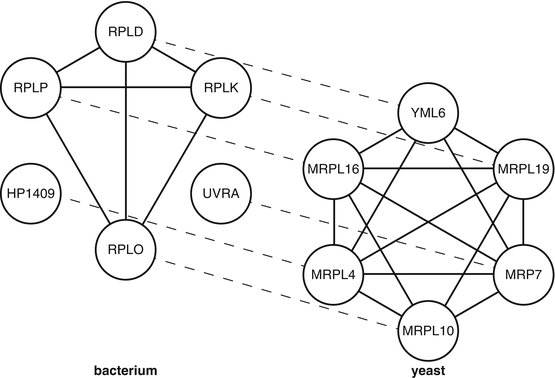
\includegraphics[
                width=0.45\linewidth,
                trim=0pt 0pt 0pt 0pt, % trim: left bottom right top
                clip
            ]{../images/graph_alignment_problem.png}
            \caption{Node alignment.}
            \source{\url{https://link.springer.com/rwe/10.1007/978-1-4419-9863-7_992}}
            % \label{fig:my_image}
        \end{figure}

        \begin{note}
            {Introduce your self}
        \end{note}
    \end{frame}

    \begin{frame}{MS dataset format}
        \begin{figure}[htp!]
            \centering
            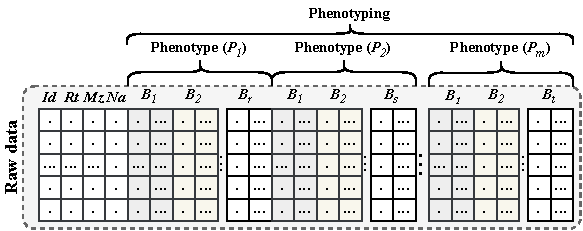
\includegraphics[
                width=0.8\linewidth,
                trim=0pt 0pt 0pt 0pt, % trim: left bottom right top
                clip
            ]{../images/raw_data.pdf}
            \caption{Aligned mass spectrometry data format.}
            % \source{Author, 2024.}
            % \label{fig:my_image}
        \end{figure}

        \begin{note}
            {Introduce your self}
        \end{note}
    \end{frame}

    \begin{frame}{Base GNN model}
        \texttt{T-GAE}: Transferable Graph Autoencoder for Network Alignment.

        \scriptsize (He, J., Kanatsoulis, C., \& Ribeiro, A., 2024)

        \begin{figure}[htp!]
            \centering
            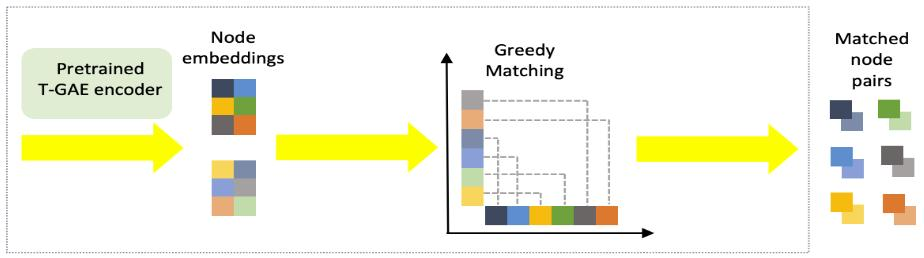
\includegraphics[
                width=0.8\linewidth,
                trim=0pt 0pt 0pt 0pt, % trim: left bottom right top
                clip
            ]{../images/T-GAE.jpg}
            \caption{\texttt{T-GAE} encoder.}
            % \source{Author, 2024.}
            % \label{fig:my_image}
        \end{figure}

        \begin{note}
            {Introduce your self}
        \end{note}
    \end{frame}

\section{Methodology}
    \begin{frame}{Methodology}
        \begin{figure}[htp!]
            \centering
            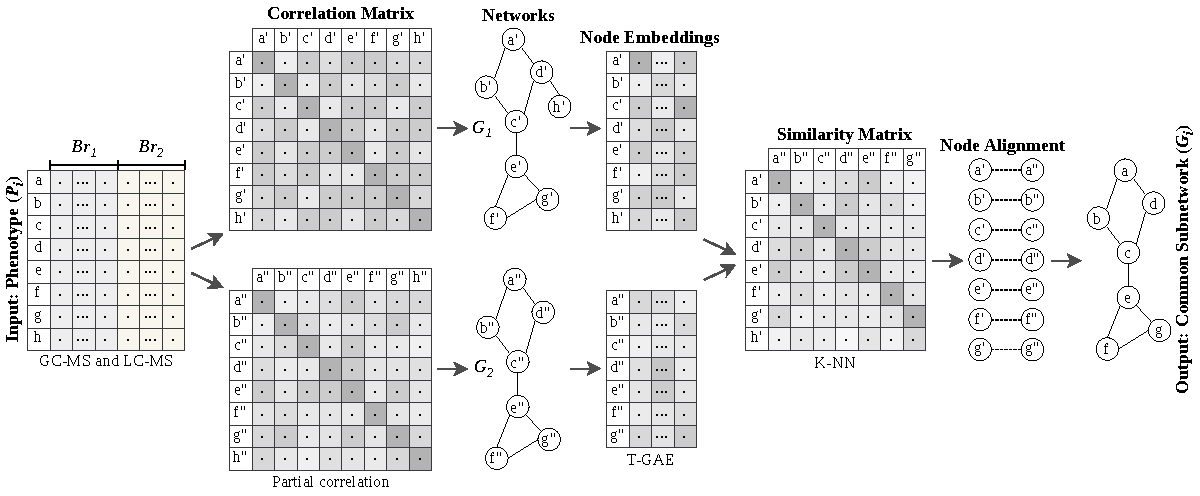
\includegraphics[
                width=1.0\linewidth,
                trim=0pt 0pt 0pt 0pt, % trim: left bottom right top
                clip
            ]{../images/Method_NA.pdf}
            \caption{Our workflow.}
            % \source{Author, 2024.}
            % \label{fig:my_image}
        \end{figure}

        \begin{note}
            {Introduce your self}
        \end{note}
    \end{frame}

\section{Experiments}

\section{Results}
    \begin{frame}{Build metabolomic networks}
        \begin{table}[htp!]
            % \scriptsize
            \centering
            \caption{Dataset information.}
            % \label{tab:table1}
            \begin{tabular}{lrrrrlr}\toprule
                Group & Subgroup & $|V|$ & $|E|$ & Density & Connected \\\midrule
                \textit{secoAmazonas} & 1 & 2071 & $1\,113\,277$ & 0.52 & True \\
                \textit{secoAmazonas} & 2 & 2071 & $1\,085\,089$ & 0.51 & True \\
                \textit{secoSanMartin} & 1 & 2069 & $1\,082\,335$ & 0.51 & True \\
                \textit{secoSanMartin} & 2 & 2071 & $1\,103\,292$ & 0.51 & True \\
                \textit{secoCusco} & 1 & 2072 & $1\,091\,447$ & 0.51 & True \\
                \textit{secoCusco} & 2 & 2072 & $1\,086\,182$ & 0.51 & True \\
                \textit{frescoCusco} & 1 & 2071 & $1\,114\,859$ & 0.52 & True \\
                \textit{frescoCusco} & 2 & 2072 & $1\,089\,225$ & 0.51 & True \\\bottomrule
            \end{tabular}
        \end{table}

        \begin{note}
            {Write your notes here}
        \end{note}
    \end{frame}

    \begin{frame}{Node embedding (T-GAE)}
        \begin{figure}[htp!]
            \centering
            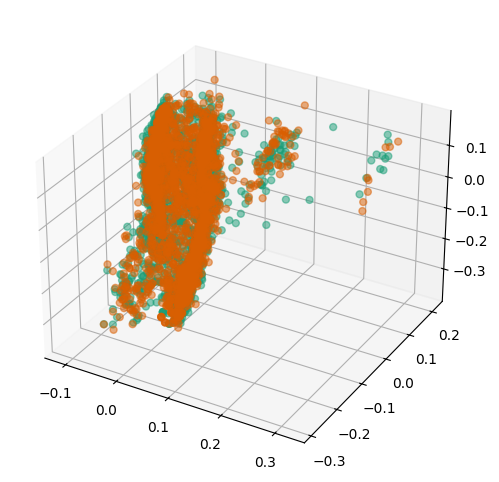
\includegraphics[
                width=0.45\linewidth,
                trim=0pt 0pt 0pt 0pt, % trim: left bottom right top
                clip
            ]{../images/secoSanMartin.png}
            \caption{Node embedding (\textit{secoSanMartin}).}
            % \source{Author, 2024.}
            % \label{fig:my_image}
        \end{figure}

        \begin{note}
            {Introduce your self}
        \end{note}
    \end{frame}

    \begin{frame}{Network alignment}
        \begin{columns}[t] % Option "c" centers vertically, while "t" aligns to the top.
            \begin{column}{0.4\textwidth}
                \begin{table}[htp!]
                    \scriptsize
                    \centering
                    \caption{Node aligment (\textit{secoSanMartin}).}
                    % \label{tab:table1}
                    \begin{tabular}{rl}\toprule
                        ID 1 & ID 2 \\\midrule
                        \rowcolor{yellow}
                        13 & 13 \\
                        19 & 252 \\
                        27 & 378 \\
                        31 & 1148 \\
                        \rowcolor{yellow}
                        38 & 38 \\
                        43 & 273 \\
                        49 & 72 \\
                        \rowcolor{yellow}
                        50 & 50 \\
                        51 & 366 \\
                        53 & 241 \\
                        73 & 270 \\
                        ... & ... \\
                        1825 & 1726 \\\bottomrule
                    \end{tabular}
                \end{table}
            \end{column}
            
            \begin{column}{0.6\textwidth}
                \begin{table}[htp!]
                    \scriptsize
                    \centering
                    \caption{Node filtered \textbf{133/2072} (\textit{secoSanMartin}).}
                    % \label{tab:table1}
                    \begin{tabular}{lrrl}\toprule
                        ID & Rt & Mz & Metabolite name \\\midrule
                        13 & 6.10 & 281.05 & Unknown \\
                        38 & 6.16 & 182.10 & Unknown \\
                        50 & 6.20 & 354.10 & Unknown \\
                        128 & 6.47 & 119.20 & Unknown \\
                        184 & 6.76 & 341.14 & Unknown \\
                        261 & 7.23 & 371.06 & Unknown \\
                        272 & 7.29 & 327.01 & Unknown \\
                        314 & 7.61 & 57.02 & DECANE; EI-B; MS \\
                        336 & 7.77 & 53.96 & Unknown \\
                        339 & 7.81 & 328.01 & Unknown \\
                        400 & 8.31 & 109.08 & CITRONELLYL ACETATE... \\ %; EI-B; MS \\
                        402 & 8.31 & 109.13 & BETA-HOMOCYCLOCITRAL... \\ %; EI-B; MS \\
                        407 & 8.37 & 401.11 & Unknown \\\bottomrule
                    \end{tabular}
                \end{table}
            \end{column}
        \end{columns}

        \begin{note}
            {Introduce your self}
        \end{note}
    \end{frame}

\section{Discussion}

\section{Conclusion}

\section*{References}
    \begin{frame}
        \begin{center}
            {\Huge\calligra Thanks!} \\
            % {\Huge\textit{Thank you for your attention!}}\\
            {\Huge $\infty$} \\
            edwin.alvarez@pucp.edu.pe \\
            \url{https://github.com/win7}
        \end{center}
    \end{frame}
    
    % Bibliography
    % \input{ref.bib}
    \begin{frame}[allowframebreaks]
        \footnotesize % use this command to resize
        % \bibliography{ref}
        % \bibliographystyle{unsrt}
        % \bibliographystyle{alpha}
        
        \begin{itemize}
            \item Erciyes, K. (2018). \textit{Guide to graph algorithms} % (pp. 15-35). Springer International Publishing.
            \item Yao Ma, Jiliang Tang. (2021). \textit{Deep Learning on Graphs}.
            \item Stamile C., Marzullo A., Deusebio E. (2021). \textit{Graph Machine Learning}.
            \item Wu, L., Cui, P., Pei, J., Zhao, L., \& Guo, X. (2022). \textit{Graph neural networks: foundation, frontiers and applications}. % In Proceedings of the 28th ACM SIGKDD conference on knowledge discovery and data mining (pp. 4840-4841).            
            % \item Knickerbocker D. (2023). \textit{Graph Network Science with Python}.
            \item Knickerbocker, D. (2023). \textit{Network Science with Python}. % Packt Publishing Ltd.
            \item Labonne, M. (2023). \textit{Hands-On Graph Neural Networks Using Python}.
            \item Broadwater, K., \& Stillman, N. (2025). \textit{Graph neural networks in action}. % Simon and Schuster.
        \end{itemize}
    \end{frame}
\end{document}